\documentclass[twoside]{article} % For LaTeX2e
\usepackage{aistats2017}
\usepackage{amsmath,amssymb,bm,bbm,upgreek,mathrsfs}
\usepackage{algorithmic,algorithm}
\usepackage[pdftex]{graphicx}
\usepackage{caption,sidecap,subcaption}
\usepackage{hyperref}
\usepackage{url}
%\documentstyle[nips14submit_09,times,art10]{article} % For LaTeX 2.09

%%%%%%%%%%%%%%%%%%%%%%%%%%%%% Useful math macros %%%%%%%%%%%%%%%%%%%%%%%%%%%%%%%
% argmax and argmin
\DeclareMathOperator*{\argmax}{arg\,max}
\DeclareMathOperator*{\argmin}{arg\,min}

%% Distributions
\newcommand{\Norm}[2]{\mathcal{N}(#1,#2)}
\newcommand{\Unif}{\mathcal{U}}
\newcommand{\Pois}[1]{\mathcal{P}\mathrm{ois}(#1)}
\newcommand{\Exp}[1]{\mathsf{Exp}(#1)}
\newcommand{\Gamm}[2]{\mathsf{Gamma}(#1,#2)}
\newcommand{\Bern}[1]{\mathcal{B}\mathrm{ern}\left(#1\right)}
\newcommand{\Binom}[2]{\mathcal{B}\mathrm{inom}(#1,#2)}
\newcommand{\Geom}[1]{\mathcal{G}\mathrm{eom}(#1)}
\newcommand{\Cat}{\mathcal{C}\mathrm{at}}
\newcommand{\Beta}[2]{\mathcal{B}\mathrm{eta}(#1,#2)}
\newcommand{\Lapl}{\mathcal{L}\mathrm{aplace}}
\newcommand{\GP}{\mathcal{GP}}
\newcommand{\DP}{\mathcal{DP}}
\newcommand{\CRP}{\mathsf{CRP}}

%% Probability
\newcommand{\E}[1]{\mathbb{E}[#1]}
\newcommand{\Cov}[2]{\mathbb{C}\mathrm{ov}(#1,#2)}
\newcommand{\given}{\, \vert \,}

%% General
\newcommand{\R}{\mathbb{R}}
\newcommand{\Z}{\mathbb{Z}}
\newcommand{\N}{\mathbb{N}}
\newcommand{\abs}[1]{\left\vert #1 \right\vert}
\newcommand{\norm}[1]{\left\vert \left \vert #1 \right\vert \right\vert}

%% Vectors
\newcommand{\bx}{\mathbf{x}}
\newcommand{\bX}{\mathbf{X}}
\newcommand{\by}{\mathbf{y}}
\newcommand{\bY}{\mathbf{Y}}
\newcommand{\ba}{\mathbf{a}}
\newcommand{\bA}{\mathbf{A}}
\newcommand{\bb}{\mathbf{b}}
\newcommand{\bB}{\mathbf{B}}
\newcommand{\bc}{\mathbf{c}}
\newcommand{\bM}{\mathbf{M}}
\newcommand{\bC}{\mathbf{C}}
\newcommand{\bQ}{\mathbf{Q}}
\newcommand{\bl}{\mathbf{l}}
\newcommand{\bem}{\mathbf{m}}
\newcommand{\bq}{\mathbf{q}}
\newcommand{\bz}{\mathbf{z}}
\newcommand{\bZ}{\mathbf{Z}}
\newcommand{\bu}{\mathbf{u}}
\newcommand{\br}{\mathbf{r}}
\newcommand{\bs}{\mathbf{s}}
\newcommand{\bw}{\mathbf{w}}
\newcommand{\bW}{\mathbf{W}}
\newcommand{\bT}{\mathbf{T}}
\newcommand{\bth}{\bm\uptheta}
\newcommand{\bTh}{\bm\Theta}
\newcommand{\bbeta}{\boldsymbol{\beta}}
\newcommand{\btheta}{\boldsymbol{\theta}}
\newcommand{\bpi}{\boldsymbol{\pi}}
\newcommand{\bphi}{\boldsymbol{\phi}}
\newcommand{\btau}{\boldsymbol{\tau}}
\newcommand{\bmu}{\boldsymbol{\mu}}
\newcommand{\blambda}{\boldsymbol{\lambda}}

%% Sets
\newcommand{\cA}{\mathcal{A}}
\newcommand{\cB}{\mathcal{B}}
\newcommand{\cZ}{\mathcal{Z}}
\newcommand{\cM}{\mathcal{M}}


\newcommand{\fix}{\marginpar{FIX}}
\newcommand{\new}{\marginpar{NEW}}

\begin{document}
\twocolumn[

\aistatstitle{A Similarity-Biased Transition Prior for Infinite HMMs}

\aistatsauthor{ Anonymous Author 1 \And Anonymous Author 2 \And Anonymous Author 3 }

\aistatsaddress{ Unknown Institution 1 \And Unknown Institution 2 \And
  Unknown Institution 3 }
% \aistatsauthor{ Colin Reimer Dawson \And Chaofan Huang \And Clayton
%   T. Morrison }

% \aistatsaddress{ Oberlin College \And Oberlin College \And The
%   University of Arizona }
]
\title{An Infinite Hidden Markov Model With Local Transitions}

\begin{abstract}
We describe a generalization of the Hierarchical Dirichlet Process Hidden Markov Model (HDP-HMM) which is able to encode prior information that state transitions are more likely between ``similar'' states.  This is accomplished by defining a similarity function on the state space, and scaling transition probabilities by pairwise similarities. This induces a global correlation structure over the transition probabilities based on the geometry induced by the similarity function.  We call this model the Hierarchical Dirichlet Process Hidden Markov Model with Local Transitions (HDP-HMM-LT). Since the conditional posterior of the transition distributions is no longer conjugate, we present an augmented data representation of the model as a Markov Jump Process in which: (1) some jump attempts fail, and (2) the probability of success is proportional to the similarity between the source and destination states. When holding times and failed transitions are reintroduced during inference, conditional conjugacy is restored, admitting exact Gibbs sampling.  Even without the LT modification, conditioning on the holding times simplifies inference for the concentration parameters of the HDP, and allows immediate generalization to Semi-Markov dynamics without additional data augmentation.  We evaluate the model and inference method on a speaker diarization task and a ``harmonic parsing'' task using four-part chorale data, as well as on several synthetic datasets, achieving favorable comparisons to existing models.

\end{abstract}

% \section{Introduction}
\label{sec:intro}
\section{Background and Related Work}

The conventional Hierarchical Dirichlet Process Hidden Markov Model
(HDP-HMM) \cite{beal2001infinite, teh2006hierarchical} 
is a prior distribution on the transition matrix of a Hidden Markov
Model with a countably infinite state space.  The rows of the
infinite matrix are coupled through their dependence on a common, discrete base measure,
itself drawn from a Dirichlet Process (DP).
The hierarchical structure ensures that, despite the infinite state
space, a common set of destination states will be reachable with high probability
from each source state.  The generative process for the HDP-HMM is the following:

Each of a countably infinite set of states, indexed by $j$, has parameters,
$\theta_j$, drawn from a base measure, $H$.  A top-level
set of state weights, $\bbeta = (\beta_1, \beta_2, \dots)$, is drawn from a stick-breaking
process ($\mathsf{GEM}$) with concentration parameter $\gamma > 0$.
\begin{equation}
\theta_j \stackrel{i.i.d.}{\sim} H \qquad \bbeta \sim \mathsf{GEM}(\gamma)
\end{equation}
The actual transition distribution, $\bpi_j$, from state $j$,
is drawn from a DP with concentration $\alpha$ and base measure $\bbeta$:
\begin{equation}
  \label{eq:1}
  \bpi_j \stackrel{i.i.d}{\sim} DP(\alpha \bbeta) \qquad j = 1, 2, \dots
\end{equation}
The hidden state sequence is then generated according to the $\pi_j$.
Let $z_t$ be the index of the chain's state at time $t$.  Then we have
\begin{equation}
  \label{eq:4}
  z_t \given z_{t-1}, \bpi_{z_{t-1}} \sim \bpi_{z_{t-1}} \qquad t = 1, 2, \dots, T
\end{equation}
where $T$ is the length of the data sequence.  Finally, the emission distribution 
for state $j$ is a function of $\theta_j$, so that we have
\begin{equation}
  \label{eq:5}
  y_t \given z_{t}, \theta_{z_t} \sim F(\theta_{z_t})
\end{equation}

A shortcoming of this model is that the generative process does not
take into account the fact that the set of source states is the same
as the set of destination states: that is, the distribution $\bpi_j$
has an element which corresponds to state $j$.  Put another way, there
is no special treatment of the diagonal of the transition matrix, so
that self-transitions are no more likely {\it a priori} than
transitions to any other state.  The Sticky HDP-HMM \cite{fox2008hdp}
addresses this issue by adding an extra mass at location $j$ to the base
measure of the DP that generates $\bpi_j$.  That is, \eqref{eq:1} is replaced by
\begin{equation}
  \label{eq:6}
  \bpi_j \sim DP(\alpha\bbeta + \kappa \delta_j).
\end{equation}
An alternative approach that treats self-transitions as special 
is the HDP Hidden Semi-Markov Model (HDP-HSMM)
\cite{johnson2013bayesian}, wherein state duration distributions are modeled
separately, and ordinary self-transitions are ruled out.  In both the
Sticky HDP-HMM and the HDP-HSMM, auxiliary latent variables are introduced to simplify
conditional posterior distributions and facilitate Gibbs sampling.
However, while both of these models have the ability to privilege
self-transitions, they contain no notion of
similarity for pairs of states that are not identical: 
in both cases, when the transition matrix
is integrated out, the prior probability of
transitioning to state $j'$ depends only on the top-level stick
weight associated with state $j'$, and not on the identity or
parameters of the previous state $j$.

The present paper makes two main contributions: first we 
define the HDP-HMM with Local Transitions (HDP-HMM-LT), in which a
similarity structure is defined on the state space, and ``similar''
states are {\em a priori} more likely to have transitions between
them.  This is accomplished by elementwise rescaling and then
renormalizing the HDP transition matrix.  A similar rescaling and
renormalization approach is taken in the Discrete Infinite Logistic
Normal (DILN) model \cite{paisley2012discrete} in the setting of topic
modeling.  There, however, the contexts and the mixture components
(topics) are distinct sets, and there is no notion of temporal
dependence.  The second contribution of the present paper 
is an augmented data technique that allows Gibbs sampling to be used.
Previous rescaled HDP models such as DILN have relied on variational
inference.

The paper is structured as follows: In section \ref{sec:model} we
define the HDP-HMM-LT.  In section \ref{sec:inference}, we develop a
straightforward Gibbs sampling algorithm 
based on an augmented data representation, the Markov
Jump Process with Failed Transitions.  In section
\ref{sec:experiments} we test the model and inference algorithm 
on synthetic data generated from similar generative models, as well as
on a speaker diarization task in which the speakers are
inter-dependent.  Finally, in section \ref{sec:discussion}, we 
conclude and discuss the relationships between the HDP-HMM-LT and
existing HMM variants.
\section{An HDP-HMM With Local Transitions}
\label{sec:model}
We wish to add to the transition model the concept of a transition to
a ``nearby'' state, where nearness of $j$ and $j'$ is a function of
$\theta_j$ and $\theta_{j'}$.  In order to accomplish this, we first
consider an alternative construction of the transition distributions,
based on the Normalized Gamma Process.

\subsection{A Normalized Gamma Process representation of the HDP-HMM}
\label{sec:normalized-gamma}

We can define a random measure, $\mu = \sum_{j=1}^{\infty} \pi_j \delta_{\theta_j}$, where 
\begin{align}
  \pi_j \stackrel{ind}{\sim} \Gamm{w_j}{1} \qquad T =
  \sum_{j=1}^{\infty} \pi_j \qquad
  \tilde{\pi}_j = \frac{\pi_j}{T} \label{eq:20}
\end{align}
and subject to the constraint that $\sum_{j\geq 1} w_j < \infty$.  It
follows \cite{paisley2012discrete, favaro2013mcmc} that $\mu$ is distributed as a Dirichlet
Process with base measure $\bw = \sum_{j=1}^{\infty} w_j \delta_{\theta_j}$.
If we draw $\bbeta$ from a stick-breaking process and then draw a
series $\{\mu_m\}_{m=1}^M$ of
i.i.d. random measures from the above process, setting $\bw =
\alpha\bbeta$ for some $\alpha > 0$, then
this defines a Hierarchical Dirichlet Process.  If, moreover, there is
one $\mu$ associated with every state $j$, then we obtain the
transition prior for the HDP-HMM, where
\begin{align}
  \label{eq:50}
  p(z_t \given z_{t-1}, \bpi) = \tilde{\pi}_{z_{t-1}z_t}
\end{align}

\subsection{Promoting ``Local" Transitions}
\label{sec:prom-local-trans}

In the preceding formulation, the $\theta_j$ and the $\pi_{jj'}$ are independent
conditioned on the top-level measure.  Our goal is to relax this
assumption, in order to incorporate possible prior knowledge
that certain ``location'' pairs, $(\theta_j, \theta_{j'})$, are more likely than others to
produce large transition weights (i.e., states adjacent in time should
tend to be similar).  This can be accomplished by scaling the elements
$\pi_{jj'}$ by a function of $(\theta_{j}, \theta_{j'})$ prior to
normalization, or equivalently letting the Gamma distribution have
a proximity-dependent rate parameter.  

Let $\Phi: \Omega \times \Omega \to [0,\infty)$ represent a
``similarity function'', and define a collection of random variables
$\{\phi_{jj'}\}_{j,j' \geq 1}$ according to $\phi_{jj'} = \phi(\theta_j, \theta_j')$.
We can then generalize \eqref{eq:20} to
\begin{align}
  \pi_{jj'} \given \bbeta, \btheta \sim \Gamm{\alpha \beta_{j'}}{\phi_{jj'}^{-1}} \qquad
  T_j = \sum_{j'=1}^{\infty} \pi_{jj'} \qquad \tilde{\pi}_{jj'} = \frac{\pi_{jj'}}{T_j}
\end{align}
so that the prior mean of $\pi_{jj'}$ is
$\alpha\beta_{j'}\phi_{jj'}$.  Since a similarity between one object
and another should not exceed the similarity between an object and
itself, and since a constant rescaling of the similarity will be
absorbed in normalization, we will assume that $0 \leq \phi_{jj'} \leq 1$ for all $j$
and $j'$.

\subsection{The HDP-HMM-LT as the Marginalization of
a Markov Jump Process with ``Failed'' Jumps}
\label{sec:dist-based-filt}

We can gain stronger intuition, as well as simplify posterior
inference, by representing the HDP-HMM-LT described in the last section
as a continuous time Markov jump process where holding times have been
integrated out.  In particular, suppose that some of the attempts to jump
from one state to another fail, and the failure probability
increases as a function of the ``distance'' between the states.

Let $\Phi$ be defined as in the last section, and let 
$\bbeta$, $\btheta$ and $\bpi$ be defined as in the Normalized Gamma
Process representation of the ordinary HDP-HMM (so,
  $\pi_{jj'} \given \bbeta, \btheta \sim \Gamm{\alpha \beta_{j'}}{1}$).
Now suppose that when the process is in state $j$, jumps to state
$j'$ are made at rate $\pi_{jj'}$.  This defines a continuous-time
Markov Process where the off-diagonal elements of the transition rate
matrix are the off diagonal elements of $\bpi$.  In addition,
self-jumps are allowed, and occur with rate $\pi_{jj}$.   If we only
observe the jumps and not the durations between jumps, this is an
ordinary Markov chain.  If we do not observe the jumps themselves, but
instead an observation is generated once per jump from a distribution that depends
on the state being jumped to, then we have an ordinary HMM.

We modify this process as follows.  
Suppose that each jump attempt from state $j$ to state $j'$ has a
chance of failing, which is an increasing function of the ``distance''
between the states.  In particular, let the success probability be
$\phi_{jj'}$ (recall that we assumed above that $0 \leq \phi_{jj'}
\leq 1$ for all $j,j'$).  Then, the rate of successful jumps from $j$
to $j'$ is $\pi_{jj'}\phi_{jj'}$, and the corresponding rate of unsuccessful jump
attempts is $\pi_{jj'}(1-\phi_{jj'})$.  We denote the overall rate of successful jumps
while in state $j$ by $T_j := \sum_{j'} \pi_{jj'} \phi_{jj'}$.
Given that the process is in state $j$ at discretized time $t$ (that is,
$z_{t} = j$), the probability that the first successful jump is to
state $j'$ (that is, $z_{t+1} = j'$) 
is proportional to the rate of successful jump attempts to $j'$, which
is $\pi_{jj'}\phi_{jj'}$.  The holding time, $\tau_{t-1}$, is
independent of $z_{t+1}$ and is distributed $\mathsf{Exp}(T_j)$.  The
total time spent in state $j$ given that it is visited $n_{j}$ times,
is then
\begin{equation}
u_j \given \bz, \bpi, \btheta \stackrel{ind}{\sim} \Gamm{n_{j\cdot}}{T_j}
\end{equation}
During this period there will be $q_{jj'}$
unsuccessful attempts to jump to state $j'$, where $q_{jj'}$ is distributed $\mathsf{Pois}(u_j
\pi_{jj'}(1 - \phi_{jj'}))$.  Incorporating
$\bu = \{u_j\}$ as augmented data simplifies the likelihood for the transition
parameters, yielding
\begin{align}
  L(\bpi, \bphi \given \bz, \bu, \bQ) &= \left(\prod_{t=1}^T p(z_{t} \given
    z_{t-1}, \bpi, \bphi)\right) \prod_{j} p(u_j \given \bz, \bpi, \bphi)
  \prod_{j'} p(q_{jj'} \given u_j \pi_{jj'}, \phi_{jj'}) \notag \\
  &\propto \prod_{j} \prod_{j'} \pi_{jj'}^{n_{jj'} + q_{jj'}} \phi_{jj'}^{n_{jj'}}
  (1-\phi_{jj'})^{q_{jj'}} e^{-\pi_{jj'}u_j} \label{eq:joint-likelihood}
\end{align}

\subsection{An HDP-HSMM-LT modification}
\label{sec:an-hsmm-modification}

We note that it is trivial to modify the HDP-HMM-LT to allow for
non-Geometric duration distributions, by simply fixing the diagonal
elements of $\bpi$ to be zero, allowing $D_t$ observations to be
emitted $i.i.d.$ according to $F(\theta_{z_t})$ at jump $t$, where $D_t$ is drawn
from a state-specific duration distribution, and sampling the
latent state sequence using a message passing algorithm suited for
HSMMs \cite{johnson2013bayesian}.  Inference for the $\bphi$ matrix
is not affected, since the diagonal elements are assumed to be 1.
Unlike in the original representation of the HDP-HSMM, there is no need to introduce
additional auxiliary variables as a result of this modification, due
to the presence of the (continuous) durations, $\bu$, which were
already needed to account for the normalization of the $\bpi$.

% \subsection{Summary}
% \label{sec:model-summary}

% We have defined the following augmented generative model for the
% HDP-H(S)MM-LT:
% \begin{align}
%   \label{eq:96}
%   \bbeta &\sim \mathrm{GEM}(\gamma) \\
%   \theta_j &\stackrel{i.i.d}{\sim} H \\
%   \pi_{jj'} \given \bbeta, \btheta &\sim \Gamm{\alpha \beta_{j'}}{1}
%   \\
%   z_{t} \given z_{t-1}, \bpi, \btheta &\sim \sum_{j}
%   \left(\frac{\pi_{z_{t-1}j}\phi_{z_{t-1}j}}{\sum_{j'}
%     \pi_{z_{t-1}j'}\phi_{z_{t-1}j'}}\right)\delta_j \\
%   u_j \given \bz, \bpi, \btheta &\stackrel{ind}{\sim}
%   \Gamm{n_{j\cdot}}{\sum_{j'} \pi_{jj'}\phi_{jj'}} \\
%   q_{jj'} \given \bu, \bpi, \btheta &\stackrel{ind}{\sim}
%   \Pois{u_j(1 - \phi_{jj'})\pi_{jj'}} \\
%   \label{eq:likelihood} \by_t \given \bz, \btheta &\sim F(\theta_{z_t})
% \end{align}

% If we are using the HSMM variant, then we simply fix $\pi_{jj}$ to 0
% for each $j$, draw
% \begin{align}
%   \label{eq:97}
%   \omega_j &\stackrel{i.i.d}{\sim} G \\
%   D_t \given \bz &\stackrel{ind}{\sim} g(\omega_{z_t}),
% \end{align}
% set
% \begin{equation}
%   \label{eq:98}
%   z^*_s = z_{\max\{T \given s \leq \sum_{t=1}^T D_t\}}
% \end{equation}
% and replace \eqref{eq:likelihood} with
% \begin{equation}
%   \label{eq:likelihood-hsmm} \by_s \given \bz, \btheta \sim F(\theta_{z^*_s})
% \end{equation}


% \section{An HDP-HMM With Local Transitions}

% The goal is to add to the transition model the concept of a transition to
% a ``nearby'' state, where nearness of $j$ and $j'$ is possibly a function of
% $\theta_j$ and $\theta_{j'}$.  In order to accomplish this, we first
% consider an alternative construction of the transition distributions,
% based on the Normalized Gamma Process representation of the Dirichlet
% Process \cite{ferguson1973bayesian}.

% \subsection{A Normalized Gamma Process representation of the HDP-HMM}
% \label{sec:normalized-gamma}

% Define a random measure, $\mu = \sum_{j=1}^{\infty} \pi_j \delta_{\theta_j}$, where 
% \begin{align}
%   \pi_j &\stackrel{ind}{\sim} \Gamm{w_j}{1} \label{eq:17}\\
%   T &= \sum_{j=1}^{\infty} \pi_j \label{eq:18}\\
%   \tilde{\pi}_j &= \frac{\pi_j}{T}   \label{eq:16}\\
%   \theta_j &\stackrel{i.i.d}{\sim} H \label{eq:19}
% \end{align}
% and subject to the constraint that $\sum_{j\geq 1} w_j < \infty$,
% which ensures that $T < \infty$ almost surely.  As
% shown by Paisley et al. (2011), for fixed $\{w_j\}$ and $\{\theta_j\}$, $\mu$ is distributed as a Dirichlet
% Process with base measure $\bw = \sum_{j=1}^{\infty} w_j \delta_{\theta_j}$.
% If we draw $\bbeta$ from a stick-breaking process and then draw a
% series $\{\mu_m\}_{m=1}^M$ of
% i.i.d. random measures from the above process, setting $\bw =
% \alpha\bbeta$ for some $\alpha > 0$, then
% this defines a Hierarchical Dirichlet Process.  If, moreover, there is
% one $\mu_m$ associated with every state $j$, then we obtain the
% HDP-HMM.

% We can thus write
% \begin{align}
%   \bbeta &\sim \mathsf{GEM}(\gamma)   \label{eq:20} \\
%   \theta_j &\stackrel{i.i.d.}{\sim} H \label{eq:21}\\
%   \pi_{jj'} &\stackrel{ind}{\sim} \Gamm{\alpha \beta_{j'}}{1} \label{eq:22}\\
%   T_j &= \sum_{j'=1}^{\infty} \pi_{jj'} \\
%   \tilde{\pi}_{jj'} &= \frac{\pi_{jj'}}{T_j} \label{eq:23},
% \end{align}
% where $\gamma$ and $\alpha$ are prior concentration hyperparameters
% for the two DP levels, where
% \begin{align}
%   \label{eq:50}
%   p(z_t \given z_{t-1}, \bpi) = \tilde{\pi}_{z_{t-1}z_t}
% \end{align}
% and the observed data
% $\{y_t\}_{t\geq 1}$ distributed as
% \begin{equation}
%   \label{eq:24}
%   y_t \given z_t \stackrel{ind}{\sim} F(\theta_{z_t})
% \end{equation}
% for some family, $F$ of probability measures indexed by values of $\theta$.

% \subsection{Promoting ``Local" Transitions}
% \label{sec:prom-local-trans}

% In the preceding formulation, the $\theta_j$ and the $\pi_{jj'}$ are independent
% conditioned on the top-level measure.  Our goal is to relax this
% assumption, in order to allow for prior knowledge
% that certain ``locations'', $\theta_j$, are more likely than others to
% produce large weights.  This can be accomplished by letting the rate
% parameter in the distribution of the $\pi_{jj'}$
% be a function of $\theta_j$ and $\theta_{j'}$.  
% Let $\Phi: \Omega \times \Omega \to [0,\infty)$ represent a
% ``similarity function'', and define a collection of random variables
% $\{\phi_{jj'}\}_{j,j' \geq 1}$ according to
% \begin{equation}
%   \phi_{jj'} = \phi(\theta_j, \theta_j')
% \end{equation}
% We can then generalize \eqref{eq:20}-\eqref{eq:23} to
% \begin{align}
%   \bbeta &\sim \mathrm{GEM}(\gamma) \\
%   \theta_j &\stackrel{i.i.d}{\sim} H \\
%   \pi_{jj'} \given \bbeta, \btheta &\sim \Gamm{\alpha \beta_{j'}}{\phi_{jj'}^{-1}} \\
%   T_j &= \sum_{j'=1}^{\infty} \pi_{jj'} \\
%   \tilde{\pi}_{jj'} &= \frac{\pi_{jj'}}{T_j}
% \end{align}
% so that the expected value of $\pi_{jj'}$ is
% $\alpha\beta_{j'}\phi_{jj'}$.  Since a similarity between one object
% and another should not exceed the similarity between an object and
% itself, we will assume that $\phi_{jj'} \leq B < \infty$ for all $j$
% and $j'$, with equality holding iff $j = j'$.  Moreover, there 
% is no loss of generality by taking $B = 1$, since a constant rescaling of
% $\phi_{jj'}$ gets absorbed in the normalization.

% The above model is equivalent to simply drawing the $\pi_{jj'}$ as in
% \eqref{eq:20} and scaling each one by $\phi_{jj'}$ prior to
% normalization.

% Unfortunately, this formulation complicates inference significantly,
% as the introduction of non-constant rate parameters to the prior on
% $\bpi$ destroys the conjugacy between $\bpi$ and $\bz$, and worse, the
% conditional likelihood function for $\bpi$ contains an infinite
% sum of the elements in a row, rendering all entries within a row
% mutually dependent.

% \subsection{The HDP-HMM-LT as a continuous-time 
% Markov Jump Process with ``failed'' jumps}
% \label{sec:dist-based-filt}

% We can gain stronger intuition, as well as simplify posterior
% inference, by re-casting the HDP-HMM-LT described in the last section
% as a continuous time Markov Jump Process where some of the attempts to jump
% from one state to another fail, and where the failure probability
% increases as a function of the ``distance'' between the states.

% Let $\Phi$ be defined as in the last section, and let 
% $\bbeta$, $\btheta$ and $\bpi$ be defined as in the Normalized Gamma
% Process representation of the ordinary HDP-HMM.  That is,
% \begin{align}
%   \label{eq:beta} \bbeta &\sim \mathrm{GEM}(\gamma) \\
%   \theta_j &\stackrel{i.i.d}{\sim} H \\
%   \pi_{jj'} \given \bbeta, \btheta &\sim \Gamm{\alpha \beta_{j'}}{1}
% \end{align}
% Now suppose that when the process is in state $j$, jumps to state
% $j'$ are made at rate $\pi_{jj'}$.  This defines a continuous-time
% Markov Process where the off-diagonal elements of the transition rate
% matrix are the off diagonal elements of $\bpi$.  In addition,
% self-jumps are allowed, and occur with rate $\pi_{jj}$.   If we only
% observe the jumps and not the durations between jumps, this is an
% ordinary Markov chain, whose transition matrix is obtained by
% appropriately normalizing $\bpi$.  If we do not observe the jumps themselves, but
% instead an observation is generated once per jump from a distribution that depends
% on the state being jumped to, then we have an ordinary HMM.

% I modify this process as follows.  
% Suppose that each jump attempt from state $j$ to state $j'$ has a
% chance of failing, which is an increasing function of the ``distance''
% between the states.  In particular, let the success probability be
% $\phi_{jj'}$ (recall that we assumed above that $0 \leq \phi_{jj'}
% \leq 1$ for all $j,j'$).  Then, the rate of successful jumps from $j$
% to $j'$ is $\pi_{jj'}\phi_{jj'}$, and the corresponding rate of unsuccessful jump
% attempts is $\pi_{jj'}(1-\phi_{jj'})$.  To see this, denote by
% $N_{jj'}$ the total number of jump attempts to $j'$ in a unit
% interval of time spent in state $j$.  Since we are assuming the
% process is Markovian, the total number of attempts is $\Pois{\pi_{jj'}}$
% distributed.  Conditioned on $N_{jj'}$, $n_{jj'}$ will be successful, where
% \begin{equation}
%   \label{eq:51}
%   n_{jj'} \given N_{jj'} \sim \Binom{N_{jj'}}{\phi_{jj'}}
% \end{equation}
% It is easy to show (and well known) that the marginal distribution of
% $n_{jj'}$ is $\Pois{\pi_{jj'}\phi_{jj'}}$, and the marginal
% distribution of $\tilde{q}_{jj'} := N_{jj'} - n_{jj'}$ is
% $\Pois{\pi_{jj'}(1-\phi_{jj'})}$.  The rate of successful jumps
% from state $j$ overall is then $T_j := \sum_{j'} \pi_{jj'} \phi_{jj'}$.

% Let $t$ index jumps, so that $z_t$ indicates the $t$th state visited
% by the process (couting self-jumps as a new time step).  Given
% that the process is in state $j$ at discretized time $t-1$ (that is,
% $z_{t-1} = j$), it is a standard property of Markov Processes that 
% the probability that the first successful jump is to state $j'$ (that is, $z_{t} = j'$) 
% is proportional to the rate of successful attempts to 
% $j'$, which is $\pi_{jj'}\phi_{jj'}$.  

% Let $\tau_{t}$ indicate the time elapsed between the $t$th and 
% and $t-1$th successful jump (where we assume that the first
% observation occurs when the first successful jump from a distinguished initial
% state is made).  We have
% \begin{equation}
%   \label{eq:52}
%   \tau_t \given z_{t-1} \sim \Exp{T_{z_{t-1}}}
% \end{equation}
% where $\tau_t$ is independent of $z_{t}$.

% During this period, there will be $\tilde{q}_{j't}$ unsuccessful attempts to
% jump to state $j'$, where
% \begin{equation}
%   \label{eq:53}
%   \tilde{q}_{j't} \given z_{t-1} \sim \Pois{\tau_t \pi_{z_{t-1}j'}(1-\phi_{z_{t-1}j'})}
% \end{equation}

% Define the following additional variables
% \begin{align}
%   \label{eq:56}
%     \mathcal{T}_j &= \{t \given z_{t-1} = j\} \\
%     q_{jj'} &= \sum_{t \in \mathcal{T}_j}
%     \tilde{q}_{j't} \\
%     u_j &= \sum_{t \in \mathcal{T}_j} \tau_t 
% \end{align}
% and let $\bQ = (q_{jj'})_{j,j' \geq 1}$ be the matrix of unsuccessful
% jump attempt counts, and $\bu = (u_j)_{j \geq 1}$ be the vector of
% the total times spent in each state.

% Since each of the $\tau_t$ with $t \in \mathcal{T}_j$ are
% i.i.d. $\Exp{T_j}$, we get the marginal distribution
% \begin{equation}
% u_j \given \bz, \bpi \btheta \stackrel{ind}{\sim} \Gamm{n_{j\cdot}}{T_j}
% \end{equation}
% by the standard property that sums of i.i.d. Exponential distributions
% has a Gamma distribution with shape equal to the number of variates in
% the sum, and rate equal to the rate of the individual exponentials.  
% Moreover, since the $\tilde{q}_{j't}$ with $t \in \mathcal{T}_j$ 
% are Poisson distributed, the total number of failed
% attempts in the total duration $u_j$ is
% \begin{equation}
%   \label{eq:60}
%   q_{jj'} \stackrel{ind}{\sim} \Pois{u_j\pi_{jj'}(1-\phi_{jj'})}.
% \end{equation}

% Thus if we marginalize out the individual $\tau_t$ and
% $\tilde{q}_{j't}$, we have a joint distribution
% over $\bz$, $\bu$, and $\bQ$, conditioned on the transition rate
% matrix $\bpi$ and the success probability matrix $\bphi$, which is
% \begin{align}
%   \label{eq:54}
%   p(\bz, \bu, \bQ \given \bpi, \btheta) &= \left(\prod_{t=1}^T p(z_{t} \given
%     z_{t-1})\right) \prod_{j} p(u_j \given \bz, \bpi, \btheta)
%   \prod_{j'} p(q_{jj'} \given u_j \pi_{jj'}, \phi_{jj'}) \\
%   &= \left(\prod_{t} \frac{\pi_{z_{t-1}z_t}\phi_{z_{t-1}z_t}}{T_{z_{t-1}}}\right) \prod_{j}
%   \frac{T_j^{n_{j\cdot}}}{\Gamma(n_{j\cdot})} u_j^{n_{j\cdot} - 1}
%   e^{-T_j u_j} \\ &\qquad\qquad\times
%   \prod_{j'} e^{-u_j\pi_{jj'}(1-\phi_{jj'})} u_j^{q_{jj'}}
%   \pi_{jj'}^{q_{jj'}} (1-\phi_{jj'})^{q_{jj'}} (q_{jj'}!)^{-1} \\
%   &= \prod_{j} \Gamma(n_{j\cdot})^{-1} u_j^{n_{j\cdot} + q_{j\cdot}-1}
%   \\ &\qquad\qquad \times \prod_{j'}
%   \pi_{jj'}^{n_{jj'} + q_{jj'}} \phi_{jj'}^{n_{jj'}}
%   (1-\phi_{jj'})^{q_{jj'}} e^{-\pi_{jj'}\phi_{jj'}u_j}
%   e^{-\pi_{jj'}(1-\phi_{jj'})u_j} (q_{jj'}!)^{-1} \\
%   &\label{eq:joint-likelihood} = \prod_{j} \Gamma(n_{j\cdot})^{-1} u_j^{n_{j\cdot} + q_{j\cdot}-1} \prod_{j'}
%   \pi_{jj'}^{n_{jj'} + q_{jj'}} \phi_{jj'}^{n_{jj'}}
%   (1-\phi_{jj'})^{q_{jj'}} e^{-\pi_{jj'}u_j} (q_{jj'}!)^{-1}
% \end{align}

% \subsection{An HDP-HSMM-LT modification}
% \label{sec:an-hsmm-modification}

% Note that it is trivial to modify the HDP-HMM-LT to allow the
% number of observations generated each time a state is visited to have
% a distribution which is not Geometric, by simply fixing the diagonal
% elements of $\bpi$ to be zero, and allowing $D_t$ observations to be
% emitted $i.i.d.$ $F(\theta_{z_t})$ at jump $t$, where
% \begin{equation}
%   \label{eq:95}
%   D_t \given \bz \stackrel{ind}{\sim} g(\omega_{z_t}) \qquad \omega_j
%   \stackrel{i.i.d}{\sim} G
% \end{equation}
% The likelihood then includes the additional term for the $D_t$, and
% the only inference step which is affected is that instead of sampling
% $\bz$ alone, we sample $\bz$ and the $D_t$ jointly, by defining
% \begin{equation}
%   z^*_s = z_{\max\{T \given s \leq \sum_{t=1}^T D_t\}}
% \end{equation}
% where $s$ ranges over the number of observations, 
% and associating a $\by_s$ with each $z^*_s$.
% Inferences about $\bphi$ are not affected, since the diagonal
% elements are assumed to be 1 anyway.

% This is the same construction used in the Hierarchical Dirichlet
% Process Hidden Semi-Markov Model (HDP-HSMM;
% \cite{johnson2013bayesian}).  
% Unlike in the standard representation of the HDP-HSMM,
% however, there is no need to introduce
% additional auxiliary variables as a result of this modification, due
% to the presence of the (continuous) durations, $\bu$, which were
% already needed to account for the normalization of the $\bpi$.

% \subsection{Summary}
% \label{sec:model-summary}

% I have defined the following augmented generative model for the
% HDP-H(S)MM-LT:
% \begin{align}
%   \label{eq:96}
%   \bbeta &\sim \mathrm{GEM}(\gamma) \\
%   \theta_j &\stackrel{i.i.d}{\sim} H \\
%   \pi_{jj'} \given \bbeta, \btheta &\sim \Gamm{\alpha \beta_{j'}}{1}
%   \\
%   z_{t} \given z_{t-1}, \bpi, \btheta &\sim \sum_{j}
%   \left(\frac{\pi_{z_{t-1}j}\phi_{z_{t-1}j}}{\sum_{j'}
%     \pi_{z_{t-1}j'}\phi_{z_{t-1}j'}}\right)\delta_j \\
%   u_j \given \bz, \bpi, \btheta &\stackrel{ind}{\sim}
%   \Gamm{n_{j\cdot}}{\sum_{j'} \pi_{jj'}\phi_{jj'}} \\
%   q_{jj'} \given \bu, \bpi, \btheta &\stackrel{ind}{\sim}
%   \Pois{u_j(1 - \phi_{jj'})\pi_{jj'}} \\
%   \label{eq:likelihood} \by_t \given \bz, \btheta &\sim F(\theta_{z_t})
% \end{align}

% If we are using the HSMM variant, then we simply fix $\pi_{jj}$ to 0
% for each $j$, draw
% \begin{align}
%   \label{eq:97}
%   \omega_j &\stackrel{i.i.d}{\sim} G \\
%   D_t \given \bz &\stackrel{ind}{\sim} g(\omega_{z_t}),
% \end{align}
% for chosen $G$ and $g$, set
% \begin{equation}
%   \label{eq:98}
%   z^*_s = z_{\max\{T \given s \leq \sum_{t=1}^T D_t\}}
% \end{equation}
% and replace \eqref{eq:likelihood} with
% \begin{equation}
%   \label{eq:likelihood-hsmm} \by_s \given \bz, \btheta \sim F(\theta_{z^*_s})
% \end{equation}

\section{Inference}
\label{sec:inference}

We develop a Gibbs sampling algorithm based on the Markov Process with
Failed Jumps representation, augmenting the data with the duration
variables $\bu$, the failed jump attempt count matrix, $\bQ$, as well
as additional auxiliary variables which we will define below.
In this representation the transition matrix is not represented
directly, but is a function of the unscaled transition matrix $\pi$
and the similarity matrix $\bphi$.  The full set of variables is
partitioned into blocks: $\{\gamma, \alpha, \bbeta, \bpi\}$,
$\{\bz, \bu, \bQ, \Lambda\}$, $\{\btheta\}$, and $\{\xi\}$, where $\Lambda$
represents a set of auxiliary variables that will be introduced
below, $\btheta$ represents the emission and state location
parameters (which may be further factored depending on the specific
choice of model), and $\xi$ represents additional
parameters such as any free parameters of the similarity function,
$\Phi$, and any hyperparameters of the emission distribution.


\subsection{Sampling Transition Parameters and Hyperparameters}

The joint posterior over $\gamma$, $\alpha$, $\bbeta$ and $\bpi$
given the other variables will factor as
\begin{equation}
  \label{eq:46}
  p(\gamma, \alpha, \bbeta, \bpi) = p(\gamma) p(\alpha) p(\bbeta \given \gamma) p(\bpi
  \given \alpha, \bbeta)
\end{equation}
where we have omitted the dependence on the augmented data,
$\mathcal{D} = (\bz, \bu, \bQ, \Lambda)$ for conciseness.  
We describe these four factors in reverse order.

\paragraph{Sampling \texorpdfstring{$\bpi$}{pi}} 
Having used data augmentation to simplify the likelihood for $\bpi$ to
the factored conjugate form in \eqref{eq:joint-likelihood}, the individual
$\pi_{jj'}$ are {\it a posteriori} independent Gamma distributed:
\begin{equation}
\pi_{jj'} \given \alpha, \beta_{j'}, \mathcal{D} \stackrel{ind}{\sim}
\Gamm{\alpha\beta_{j'} + n_{jj'} + q_{jj'}}{1 + u_j} \qquad j,j' \geq 1
\end{equation}

\paragraph{Sampling \texorpdfstring{$\bbeta$}{beta}}
\label{sec:sampling-bbeta}
To enable joint sampling of the latent state sequence, we employ a
weak limit approximation to the HDP \cite{johnson2013bayesian}, approximating the stick-breaking
process for $\bbeta$ using a finite Dirichlet distribution with a
finite number of components, $J$, which is larger than we expect to
need.  Due to the product of Gammas form, we can integrate out $\bpi$ 
analytically from $p(\bpi, \mathcal{D} \given \bbeta)$, to obtain the
the marginal likelihood for $\bbeta$.  Together, we have
\begin{align}
\label{eq:beta-prior-likelihood}
  p(\bbeta \given \gamma) = \frac{\Gamma(\gamma /
    J)^J}{\Gamma(\gamma)} \prod_{j} \beta_{j}^{\frac{\gamma}{J} - 1} \qquad
  p(\mathcal{D} \given \bbeta, \alpha) \propto
  \prod_{j=1}^J (1+u_j)^{-\alpha} \prod_{j'}
    \frac{\Gamma(\alpha\beta_{j'} + n_{jj'} +
    q_{jj'})}{\Gamma(\alpha\beta_{j'})} 
\end{align}
 where we have used the fact that the $\beta_j$ sum to 1 to pull out
 terms of the form $(1 + u_j)^{-\alpha\beta_{j'}}$ from the inner
 product in the likelihood.  Following Teh et al. (2006), 
we can introduce auxiliary variables $\{m_{jj'}\}$, with
\begin{equation}
  \label{eq:m-distribution}
  p(m_{jj'} \given \beta_{j'}, \alpha, \mathcal{D}) \stackrel{ind}{\propto}
  s(n_{jj'} + q_{jj'}, m_{jj'}) \alpha^{m_{jj'}}
    \beta_{j'}^{m_{jj'}}
\end{equation}
for integer $m_{jj'}$ ranging between $0$ and $n_{jj'} + q_{jj'}$,
where $s(n,m)$ is an unsigned Stirling number of the first kind.
The normalizing constant in this distribution cancels the ratio of
Gamma functions in the $\bbeta$ likelihood, so, letting $m_{\cdot j} =
\sum_{j'} m_{j'j}$, we obtain simply
\begin{equation}
  \label{eq:beta-posterior}
  \bbeta \given \bM, \gamma \sim \mathrm{Dirichlet}(\frac{\gamma}{J} +
  m_{\cdot 1}, \dots, \frac{\gamma}{J} + m_{\cdot J})
\end{equation}

\paragraph{Sampling Concentration Parameters}
\label{sec:sampling-alpha}
After incorporating $\bM$ into $\mathcal{D}$, we can integrate out
$\bbeta$, from the joint likelihood $p(\bbeta,\mathcal{D} \given \gamma, \alpha)$:
\begin{align}
\label{eq:gamma-marginal-likelihood}
  p(\mathcal{D} \given \alpha, \gamma) \propto
  \alpha^{m_{\cdot\cdot}} e^{-\sum_{j''} \log(1+u_{j''}) \alpha}
  \frac{\Gamma(\gamma)}{\Gamma(\gamma + m_{\cdot\cdot})}
  \prod_j
  \frac{\Gamma(\frac{\gamma}{J} + m_{\cdot
      j})}{\Gamma(\frac{\gamma}{J}) } 
\end{align}
Assume that $\alpha$ and $\gamma$ have Gamma priors.  Then
the update to alpha is conjugate,
\begin{equation}
  \label{eq:alpha-posterior}
  \alpha \given \mathcal{D} \sim \Gamm{a_{\alpha}
    + m_{\cdot\cdot}}{b_\alpha + \sum_j\log(1+u_j)},
\end{equation}
and to simplify the likelihood for $\gamma$, we can introduce a final
set of auxiliary variables, $\br = (r_1, \dots,
r_J)$, $r_j \in \{0,\dots,m_{\cdot j}\}$ and $t \in (0,1)$ with the following distributions:
\begin{align}
  \label{eq:9}
  p(r_j \given m_{\cdot j}, \gamma) \propto s(m_{\cdot j}, r)
    \left(\frac{\gamma}{J}\right)^r \qquad
  p(t \given m_{\cdot\cdot} \gamma) \propto 
    t^{\gamma - 1} (1-t)^{m_{\cdot\cdot} - 1}.
\end{align}
The normalizing constants are ratios of Gamma functions, which cancel
those in \eqref{eq:gamma-marginal-likelihood}, so that
\begin{equation}
  \label{eq:18}
  \gamma \given \mathcal{D} \sim \Gamm{a_{\gamma} + r_{\cdot}}{b_{\gamma} - \log(t)}
\end{equation}

\subsection{Sampling \texorpdfstring{$\bz$}{the latent state sequece} and the auxiliary variables}
\label{sec:sampling-z_t}

We sample the hidden state sequence, $\bz$, jointly with the auxiliary
variables, which consist of $\bu$, $\bQ$, $\bM$, $\br$ and $t$.  The
joint conditional distribution of these variables is defined directly
by the generative model:
\begin{align}
  \label{eq:19}
  p(\mathcal{D}) = p(\bz) p(\bu \given \bz) p(\bQ \given
  \bu) p(\bM \given \bz, \bQ) p(\br \given \bM) p(t
  \given\bM)
\end{align}
Since we are conditioning on the transition matrix, we can
sample the entire sequence $\bz$ at once with the forward-backward algorithm,
as in an ordinary HMM, or its corresponding generalization if we are
using the HSMM variant.  Having done this, we can sample $\bu$, $\bQ$, $\bM$,
$\br$ and $t$ from their forward distributions.

\subsection{Sampling state and emission parameters}
\label{sec:sampling-eta}

Depending on the application, the similarities $\{\phi_{jj'}\}$ may be based
directly on the emission distributions, or may be based on a separate set
of variables.  In the experiments described below we assume the
former.  For simplicity, we denote the collection of these variables
by $\btheta$.  We have two likelihood components:
\begin{align}
  \label{eq:65}
  p(\bz, \bQ \given \btheta) \propto \prod_{j}\prod_{j'}
  \phi_{jj'}^{n_{jj'}}(1-\phi_{jj'})^{q_{jj'}} \qquad
  p(\bY \given \bz, \btheta) = \prod_{t=1}^T f(\by_t; \theta_{z_t})
\end{align}
where proportionality is with respect to variation in $\btheta$.

% \section{Inference}
% \label{sec:inference}

% I develop a Gibbs sampling algorithm based on the Markov Process with
% Failed Jumps representation, augmenting the data with the duration
% variables $\bu$, the failed jump attempt count matrix, $\bQ$, as well
% as additional auxiliary variables which we will define below.
% In this representation the transition matrix is not modeled
% directly, but is a function of the unscaled transition matrix $\pi$
% and the similarity matrix $\bphi$.  The full set of variables is
% partitioned into three blocks: $\{\gamma, \alpha, \bbeta, \bpi\}$,
% $\{\bz, \bu, \bQ, \Lambda\}$, and $\{\btheta\}$, where $\Lambda$
% represents a set of auxiliary variables that will be introduced
% below.  The variables in each block are sampled jointly 
% conditioned on the other two blocks.

% Since we are representing the transition matrix of the Markov chain
% explicitly, we approximate the stick-breaking process that produces
% $\bbeta$ using a finite Dirichlet distribution with a number of 
% components larger than we expect to need, forcing the remaining 
% components to have zero weight.  
% Let $J$ indicate the maximum number of states.  Then,
% we approximate \eqref{eq:beta} with
% \begin{equation}
%   \label{eq:28}
%   \bbeta \given \gamma \sim \mathrm{Dirichlet}(\gamma / J, \dots,
%   \gamma / J)
% \end{equation}
% This distribution converges weakly to the Stick-Breaking Process as $J \to
% \infty$.  In practice, $J$ is large enough when the vast majority of the
% probability mass in $\bbeta$ is allocated to a strict subset of
% components, or when the latent state sequence $\bz$ never uses all $J$
% available states, indicating that the data is well described by a number of
% states less than $J$.

% \subsection{Sampling Transition Parameters and Hyperparameters}
% \label{sec:sampling-pi}

% The joint conditional over $\gamma$, $\alpha$, $\bbeta$ and $\bpi$
% given $\bz$, $\bu$, $\bQ$, $\Lambda$ and $\btheta$ will factor as
% \begin{equation}
%   \label{eq:46}
%   p(\gamma, \alpha, \bbeta, \bpi \given \bz, \bu, \bQ, \Lambda, \btheta) = p(\gamma \given
%   \Lambda) p(\alpha \given \Lambda) p(\bbeta \given \gamma, \Lambda) p(\bpi
%   \given \alpha, \bbeta, \btheta, \bz)
% \end{equation}
% I will derive these four factors in reverse order.

% \subsubsection{Sampling \texorpdfstring{$\bpi$}{pi}}

% The entries in $\bpi$ are conditionally independent given $\alpha$ and
% $\bbeta$, so we have the prior
% \begin{equation}
%   \label{eq:47}
%   p(\bpi \given \bbeta, \alpha) = \prod_{j} \prod_{j'}
%   \Gamma(\alpha\beta_{j'})^{-1}
%   \pi_{jj'}^{\alpha\beta_{j'} - 1} \exp(-\pi_{jj'}),
% \end{equation}
% and the likelihood given augmented data $\{\bz, \bu, \bQ\}$ given by
% \eqref{eq:joint-likelihood}.  Combining these, we have
% \begin{equation}
%   \label{eq:61}
%   p(\bpi, \bz, \bu, \bQ \given \bbeta, \alpha, \btheta) =
%   \prod_{j} u_j^{n_{j\cdot} + q_{j\cdot}
%   - 1}\prod_{j'} 
%   \Gamma(\alpha\beta_{j'})^{-1} \pi_{jj'}^{\alpha\beta_{j'} + n_{jj'}
%     + q_{jj'} - 1} e^{-(1 + u_j)
%     \pi_{jj'}} \phi_{jj'}^{n_{jj'}} (1-\phi_{jj'})^{q_{jj'}} (q_{jj'}!)^{-1}
% \end{equation}
% Conditioning on everything except $\bpi$, we get
% \begin{align}
%   \label{eq:24}
%   p(\bpi \given \bQ, \bu, \bZ, \bbeta, \alpha, \btheta) &\propto \prod_j
%   \prod_{j'} \pi_{jj'}^{\alpha\beta_{j'} + n_{jj'} + q_{jj'} - 1}
%   \exp(-(1 + u_j)\pi_{jj'})
% \end{align}
% and thus we see that the $\pi_{jj'}$ are conditionally independent
% given $\bu$, $\bZ$ and $\bQ$, and distributed according to
% \begin{align}
%   \label{eq:25}
%   \pi_{jj'} \given n_{jj'}, q_{jj'}, \beta_{j'}, \alpha \stackrel{ind}{\sim}
%   \Gamm{\alpha\beta_{j'} + n_{jj'} + q_{jj'}}{1 + u_j}
% \end{align}


% \subsubsection{Sampling \texorpdfstring{$\bbeta$}{beta}}
% \label{sec:sampling-bbeta}

% Consider the conditional distribution of $\bbeta$ having
% integrated out $\bpi$.  The prior density of $\bbeta$ from
% \eqref{eq:28} is
% \begin{equation}
%   \label{eq:62}
%   p(\bbeta \given \gamma) =
%   \frac{\Gamma(\gamma)}{\Gamma(\frac{\gamma}{J})^J} \prod_{j}
%   \beta_j^{\frac{\gamma}{J} - 1}
% \end{equation}
% After integrating out $\bpi$ in \eqref{eq:61}, we have
% \begin{align}
%   p(\bz, \bu, \bQ \given \bbeta, \alpha, \gamma, \btheta) &=
%   \prod_{j=1}^J u_{j} ^{-1}
%   \prod_{j'=1}^J u^{n_{jj'} + q_{jj'} - 1}(1 +
%   u_j)^{-(\alpha\beta_{j'} + n_{jj'} + q_{jj'})}
%   \\
%   &\qquad \qquad \times \frac{\Gamma(\alpha\beta_{j'} + n_{jj'} +
%     q_{jj'})}{\Gamma(\alpha\beta_{j'})} \phi_{jj'}^{n_{jj'}}(1-\phi_{jj'})^{q_{jj'}}
%   (q_{jj'}!)^{-1} \\
%   &= \prod_{j=1}^J \Gamma(n_{j\cdot})^{-1} u_j^{-1}(1+u_j)^{-\alpha}
%   \left(\frac{u_j}{1+u_j}\right)^{n_{j\cdot} + q_{j\cdot}} \\ &\qquad
%   \qquad \times \prod_{j' =
%     1}^J \frac{\Gamma(\alpha\beta_{j'} + n_{jj'} +
%     q_{jj'})}{\Gamma(\alpha\beta_{j'})} \phi_{jj'}^{n_{jj'}}(1-\phi_{jj'})^{q_{jj'}}
%   (q_{jj'}!)^{-1}
% \end{align}
%  where we have used the fact that the $\beta_j$ sum to 1.  Therefore
% \begin{align}
%   p(\bbeta \given \bz, \bu, \bQ, \alpha, \gamma, \btheta) &\propto \prod_{j=1}^J
%   \beta_j^{\frac{\gamma}{J} - 1} \prod_{j'=1}^J \frac{\Gamma(\alpha\beta_{j'} +
%     n_{jj'} + q_{jj'})}{\Gamma(\alpha\beta_{j'})}.
% \end{align}

% Following \cite{teh2006hierarchical}, we can write the ratios of Gamma functions
% as polynomials in $\beta_j$, as
% \begin{equation}
%   \label{eq:31}
%   p(\bbeta \given \bz, \bu, \bQ, \alpha, \gamma, \btheta) \propto \prod_{j=1}^J
%   \beta_j^{\frac{\gamma}{J} - 1} \prod_{j'=1}^{J} \sum_{m_{jj'} = 1}^{n_{jj'}}
%   s(n_{jj'} + q_{jj'}, m_{jj'}) (\alpha \beta_{j'})^{m_{jj'}}
% \end{equation}
% where $s(m,n)$ is an unsigned Stirling number of the first kind.
% This admits an augmented data representation, where we introduce a
% random matrix $\bM = (m_{jj'})_{1 \leq j,j' \leq J}$, whose
% entries are conditionally independent given $\bbeta$, $\bQ$ and $\bz$, with
% \begin{equation}
%   \label{eq:32}
%   p(m_{jj'} = m \given \beta_{j'}, \alpha, n_{jj'}, q_{jj'}) =
%   \frac{s(n_{jj'} + q_{jj'}, m) \alpha^{m}
%     \beta_{j'}^{m}}{\sum_{m'=0}^{n_{jj'} + q_{jj'}} s(n_{jj'} +
%   q_{jj'}, m') \alpha^{m'} \beta_{j'}^{m'}}
% \end{equation}
% for integer $m$ ranging between $0$ and $n_{jj'} + q_{jj'}$.  Note
% that $s(n,0) = 0$ if $n > 0$, $s(0,0) = 1$ and $s(0,m) = 0$ if $m > 0$.
% Then, we have joint distribution
% \begin{equation}
%   \label{eq:33}
%   p(\bbeta, \bM \given \bz, \bu, \bQ, \alpha, \gamma, \btheta) \propto \prod_{j=1}^J
%   \beta_j^{\frac{\gamma}{J} - 1} \prod_{j'=1}^{J} s(n_{jj'} + q_{jj'}, m_{jj'}) \alpha^{m_{jj'}} \beta_{j'}^{m_{jj'}}
% \end{equation}
% which yields \eqref{eq:31} when marginalized over $\bM$.  Again discarding
% constants in $\bbeta$ and regrouping yields
% \begin{equation}
%   \label{eq:34}
%   p(\bbeta \given \bM, \bZ, \bu, \btheta, \alpha, \gamma) \propto \prod_{j=1}^J
%   \beta_j^{\frac{\gamma}{J} + m_{\cdot j}- 1}
% \end{equation}
% which is Dirichlet:
% \begin{equation}
%   \label{eq:38}
%   \bbeta \given \bM, \gamma \sim \mathrm{Dirichlet}(\frac{\gamma}{J} +
%   m_{\cdot 1}, \dots, \frac{\gamma}{J} + m_{\cdot J})
% \end{equation}

% \subsubsection{Sampling Concentration Parameters}
% \label{sec:sampling-alpha}
% Assume that $\alpha$ and $\gamma$ have Gamma priors, with
% \begin{align}
%   \label{eq:42}
%   p(\alpha) &= \frac{b_{\alpha}^{a_{\alpha}}}{\Gamma(a_{\alpha})}
%   \alpha^{a_{\alpha} - 1} \exp(-b_{\alpha}\alpha) \\
%   p(\gamma) &= \frac{b_{\gamma}^{a_\gamma}}{\Gamma(a_{\gamma})}
%   \gamma^{a_{\gamma - 1}} \exp(-b_{\gamma}\gamma)
% \end{align}

% Having integrated out $\bpi$, we have
% \begin{align}
%   p(\bbeta, \bz, \bu, \bQ, \bM \given \alpha, \gamma, \btheta) &=
%   \frac{\Gamma(\gamma)}{\Gamma(\frac{\gamma}{J})^J} \alpha^{m_{\cdot\cdot}} \prod_{j=1}^J \beta_j^{\frac{\gamma}{J} +
%     m_{\cdot j} - 1}\Gamma(n_{j\cdot})^{-1} u_j^{-1}(1+u_j)^{-\alpha}
%   \left(\frac{u_j}{1+u_j}\right)^{n_{j\cdot} + q_{j\cdot}} \\ &\qquad
%   \qquad \times \prod_{j' =
%     1}^J s(n_{jj'} + q_{jj'}, m_{jj'}) \phi_{jj'}^{n_{jj'}}(1-\phi_{jj'})^{q_{jj'}}
%   (q_{jj'}!)^{-1}
% \end{align}
% We can also integrate out $\bbeta$, to yield
% \begin{align}
%   p(\bz, \bu, \bQ, \bM \given \alpha, \gamma, \btheta) &=
%   \alpha^{m_{\cdot\cdot}} e^{-\sum_{j''} \log(1+u_{j''}) \alpha}
%   \frac{\Gamma(\gamma)}{\Gamma(\gamma + m_{\cdot\cdot})} \\ &\qquad
%   \qquad \times \prod_j
%   \frac{\Gamma(\frac{\gamma}{J} + m_{\cdot
%       j})}{\Gamma(\frac{\gamma}{J}) \Gamma(n_{j\cdot})} u_j^{-1}
%   \left(\frac{u_j}{1+u_j}\right)^{n_{j\cdot} + q_{j\cdot}} \\ &\qquad
%   \qquad \times \prod_{j' =
%     1}^J s(n_{jj'} + q_{jj'}, m_{jj'}) \phi_{jj'}^{n_{jj'}}(1-\phi_{jj'})^{q_{jj'}}
%   (q_{jj'}!)^{-1}
% \end{align}
% demonstrating that $\alpha$ and $\gamma$ are independent given $\btheta$
% and the augmented data, with
% \begin{equation}
%   \label{eq:43}
%   p(\alpha \given \bz, \bu, \bQ, \bM, \btheta) \propto
%   \alpha^{a_{\alpha} + m_{\cdot\cdot}}\exp(-(b_\alpha + \sum_{j}\log(1+u_j))\alpha)
% \end{equation}
% and
% \begin{align}
%   \label{eq:8}
%   p(\gamma \given \bz, \bu, \bQ, \bM, \btheta) &\propto \gamma^{a_{\gamma - 1}}
%   \exp(-b_{\gamma}\gamma) \frac{\Gamma(\gamma)\prod_{j=1}^J
%     \Gamma(\frac{\gamma}{J} + m_{\cdot j})}{\Gamma(\frac{\gamma}{J})^J\Gamma(\gamma + m_{\cdot\cdot})}
% \end{align}
% So we see that
% \begin{equation}
%   \label{eq:44}
%   \alpha \given \bz, \bu, \bQ, \bM, \btheta \sim \Gamm{a_{\alpha}
%     + m_{\cdot\cdot}}{b_\alpha + \sum_j\log(1+u_j)}
% \end{equation}
% To sample $\gamma$, we introduce a new set of auxiliary variables, $\br = (r_1, \dots,
% r_j)$ and $t$ with the following distributions:
% \begin{align}
%   \label{eq:9}
%   p(r_j = r \given m_{\cdot j}, \gamma) &=
%   \frac{\Gamma(\frac{\gamma}{J})}{\Gamma(\frac{\gamma}{J}
%     + m_{\cdot j})} s(m_{\cdot j}, r)
%     \left(\frac{\gamma}{J}\right)^r \qquad r  = 1, \dots, m_{\cdot j} \\
%   p(t \given m_{\cdot\cdot} \gamma) &= \frac{\Gamma(\gamma +
%     m_{\cdot\cdot})}{\Gamma(\gamma) \Gamma(m_{\cdot\cdot})} t^{\gamma
%     - 1} (1-t)^{m_{\cdot\cdot} - 1} \qquad t \in (0,1)
% \end{align}
% so that
% \begin{align}
%   \label{eq:10}
%   p(\gamma, \br, t \given \bM) &\propto \gamma^{a_{\gamma - 1}}
%   \exp(-b_{\gamma}\gamma) t^{\gamma - 1}(1-t)^{m_{\cdot\cdot} +
%     q_{\cdot} - 1} \prod_{j=1}^J s(m_{\cdot j} + q_j, r_j)
%   \left(\frac{\gamma}{J}\right)^{r_j}
% \end{align}
% and
% \begin{align}
%   \label{eq:11}
%   p(\gamma \given \br, t) \propto \gamma^{a_\gamma +
%     r_{\cdot} - 1} \exp(-(b_{\gamma} - \log(t)) \gamma),
% \end{align}
% which is to say
% \begin{equation}
%   \label{eq:18}
%   \gamma \given \br, t, \bz, \bu, \bQ, \bM, \btheta \sim \Gamm{a_{\gamma} + r_{\cdot}}{b_{\gamma} - \log(t)}
% \end{equation}

% \subsubsection{Summary}

% I have made the following additional assumptions about the generative
% model in this section:
% \begin{equation}
%   \label{eq:100}
%   \gamma \sim \Gamm{a_{\gamma}}{b_{\gamma}} \qquad \alpha \sim \Gamm{a_{\alpha}}{b_{\alpha}}
% \end{equation}

% The joint conditional over $\gamma$, $\alpha$, $\bbeta$ and $\bpi$
% given $\bz$, $\bu$, $\bQ$, $\bM$, $\br$, $t$ and $\btheta$ factors as
% \begin{equation}
%   \label{eq:46}
%   p(\gamma, \alpha, \bbeta, \bpi \given \bz, \bu, \bQ, \br, t,
%   \btheta) = p(\gamma \given \br, t) p(\alpha \given \bu, \bM) p(\bbeta
%   \given \gamma, \bM) p(\bpi \given \alpha, \bbeta, \bz, \bu, \bQ)
% \end{equation}
% where
% \begin{align}
%   \label{eq:64}
%   \gamma \given \br, t &\sim \Gamm{a_{\gamma} + r_{\cdot}}{b_{\gamma} -
%     \log(t)} \\
%   \alpha \given \bu, \bM &\sim \Gamm{a_{\alpha} +
%     m_{\cdot\cdot}}{b_{\alpha} + \sum_j \log(1 + u_j)} \\
%   \bbeta \given \gamma, \bM &\sim \mathrm{Dirichlet}(\frac{\gamma}{J} + m_{\cdot 1},
%   \dots, \frac{\gamma}{J} + m_{\cdot J}) \\
%   \pi_{jj'} \given \alpha, \beta_{j'}, \bz, \bu, \bQ
%   &\stackrel{ind}{\sim} \Gamm{\alpha\beta_{j'} + n_{jj'} + q_{jj'}}{1 +
%   u_j}
% \end{align}


% \subsection{Sampling \texorpdfstring{$\bz$}{the latent state sequece} and the auxiliary variables}
% \label{sec:sampling-z_t}

% The hidden state sequence, $\bz$, is sampled jointly with the auxiliary
% variables, which consist of $\bu$, $\bM$, $\bQ$, $\br$ and $t$.  The
% joint conditional distribution of these variables is defined directly
% by the generative model:
% \begin{align}
%   \label{eq:19}
%   p(\bz, \bu, \bQ, \bM, \br, t \given \bpi, \bbeta, \alpha, \gamma,
%   \btheta) &= p(\bz \given \bpi, \btheta) p(\bu \given \bz, \bpi, \btheta) p(\bQ \given
%   \bu, \bpi, \btheta) p(\bM \given
%   \bz, \bQ, \alpha, \bbeta) \\
%   &\qquad \times p(\br \given
%   \gamma, \bM) p(t \given \gamma, \bM)
% \end{align}
% Since we are representing the transition matrix explicitly, we can
% sample the entire sequence $\bz$ at once with the forward-backward algorithm,
% as in an ordinary HMM (or, if we are employing the HSMM variant
% described in Sec. \ref{sec:an-hsmm-modification}, then we can use the
% modified message passing scheme for HSMMs described by
% \cite{johnson2013bayesian}.  
% Having done this, we can sample $\bu$, $\bQ$, $\bM$,
% $\br$ and $t$ from their forward distributions.  To summarize,
% we have
% \begin{align}
%   \label{eq:48}
%   u_j \given \bZ, \bpi, \btheta &\stackrel{ind}{\sim}
%   \Gamm{n_{j\cdot}}{\sum_{j'} \pi_{jj'}\phi_{jj'}} \\
%   q_{jj'} \given u_j, \pi_{jj'}, \phi_{jj'} &\stackrel{ind}{\sim}
%   \Pois{u_j(1 - \phi_{jj'})\pi_{jj'}} \\
%   m_{jj'} \given n_{jj'}, q_{jj'}, \beta_{j'}, \alpha &\stackrel{ind}{\sim}
%   \frac{\Gamma(\alpha\beta_j)}{\Gamma(\alpha\beta_j + n_{jj'} +
%     q_{jj'})}\sum_{m=1}^{n_{jj'} + q_{jj'}} s(n_{jj'} + q_{jj'}, m) \alpha^m \beta_{j'}^m \delta_{m}
%   \\
%   r_j \given m_{\cdot j}, \gamma &\stackrel{ind}{\sim}
%   \frac{\Gamma(\frac{\gamma}{J})}{\Gamma(\frac{\gamma}{J} + m_{\cdot
%       j})} \sum_{r=1}^{m_{j\cdot}} s(m_{\cdot j}, r)
%   \left(\frac{\gamma}{J}\right)^r \delta_r \\
%   t \given \gamma, \bM &\sim \Beta{\gamma}{m_{\cdot\cdot}}
% \end{align}

% \subsection{Sampling state and emission parameters}
% \label{sec:sampling-eta}

% The state parameters, $\btheta$, influence the transition matrix,
% $\bpi$ and the auxiliary vector $q$ through the similarity matrix
% matrix $\bphi$, and also control the emission distributions.
% We have likelihood factors
% \begin{align}
%   \label{eq:65}
%   p(\bz, \bQ \given \btheta) &\propto \prod_{j}\prod_{j'}
%   \phi_{jj'}^{n_{jj'}}(1-\phi_{jj'})^{q_{jj'}} \\
%   p(\bY \given \bz, \btheta) &= \prod_{t=1}^T f(\by_t; \theta_{z_t})
% \end{align}
% where proportionality is with respect to variation in $\btheta$.

% The parameter space for the hidden states, 
% the associated prior $H$ on $\btheta$, and the similarity function
% $\Phi$, is application-specific, but we consider here the case where a state,
% $\theta_j$, consists of a finite-length binary vector, motivated by the
% application of inferring the set of relevant entities in each sentence of
% a text document.

% Let $\theta_j = (\theta_{j1}, \dots, \theta_{jD})$, with $\theta_{jd} = 1$
% indicating presence of feature $d$ in context state $j$, and
% $\theta_{jd} = 0$ indicating absence.  Of course, in this case,
% the set of possible states is finite, and so on its face it may
% seem that a nonparametric model is unnecessary.  However, if $D$ is
% reasonably large, it is likely that most of the $2^D$ possible states
% are vanishingly unlikely (and, in fact, the number of observations may
% well be less than $2^D$), and so we would like a model that encourages
% the selection of a sparse set of states.  Moreover, there may be more
% than one state with the same $\theta$, but with different transition dynamics.

% \subsubsection{Sampling \texorpdfstring{$\btheta$}{latent state vectors}}
% \label{sec:sampling-eta}

% In principle, $H$ can be any distribution over binary vectors, but we
% will suppose for simplicity that it can be factored into $D$
% independent coordinate-wise Bernoulli variates.  Let $\mu_d$ be the
% Bernoulli parameter for the $d$th coordinate.

% We require a similarity function, $\Phi(\theta_j, \theta_{j'})$, which 
% varies between 0 to 1, and is equal to 1 if and only if $\theta_j =
% \theta_{j'}$.  A natural choice in this setting is the Laplacian kernel:
% \begin{align}
%   \label{eq:39}
%   \phi_{jj'} &= \Phi(\theta_j, \theta_{j'}) = \exp(-\lambda \Delta_{jj'})
% \end{align}
% where $\Delta_{jj'd} = \abs{\theta_{jd} - \theta_{j'd}}$, $\Delta_{jj'} =
% \sum_{d=1}^D \Delta_{jj'}$ is the Hamming
% distance between $\theta_j$ and $\theta_{j'}$,
% and $\lambda \geq 0$ (if $\lambda = 0$, the $\phi_{jj'}$
% are identically 1, and so do not have any influence, reducing the
% model to an ordinary HDP-HMM).

% Let
% \begin{align}
%   \label{eq:68}
%   \phi_{jj'-d} &= \exp(-\lambda(\Delta_{jj'} - \Delta_{jj'd}))
% \end{align}
% so that $\phi_{jj'} = \phi_{jj'-d} e^{-\lambda\Delta_{jj'd}}$.

% Since the matrix $\bphi$ is assumed to be symmetric, we have
% \begin{align}
%   \label{eq:70}
%   \frac{p(\bz, \bQ \given \theta_{jd}  = 1, \btheta\setminus\theta_{jd}
%     )}{p(\bz, \bQ \given \theta_{jd}  = 0, \btheta\setminus\theta_{jd} )}
%   &\propto \prod_{j' \neq j}
%   \frac{e^{-\lambda(n_{jj'} + n_{j'j})\abs{1 - \theta_{j'd}}}(1 -
%     \phi_{jj'-d} e^{-\lambda\abs{1 - \theta_{j'd}}})^{q_{jj'} +
%       q_{j'j}}}{e^{-\lambda(n_{jj'} + n_{j'j})\abs{\theta_{j'd}}}
%     (1-\phi_{jj'-d}e^{-\lambda\abs{\theta_{j'd}}})^{q_{jj'} +
%       q_{j'j}}} \\
%   &= \label{eq:71} e^{-\lambda(c_{jd0} - c_{jd1})}
%   \prod_{j' \neq j} \left(\frac{1 - \phi_{jj'-d}e^{-\lambda}}{1-\phi_{jj'-d}}\right)^{(-1)^{\theta_{j'd}}(q_{jj'} + q_{j'j})}
% \end{align}
% where $c_{jd0}$ and $c_{jd1}$ are the number of successful jumps to or
% from state $j$, to or from states with a 0 or 1, respectively, in
% position $d$.  That is,
% \begin{equation}
%   \label{eq:72}
%   c_{jd0} = \sum_{\{j' \given \theta_{j'd} = 0\}} n_{jj'} + n_{j'j}\qquad c_{jd1} = \sum_{\{j' \given \theta_{j'd} = 1\}} n_{jj'} + n_{j'j}
% \end{equation}

% Therefore, we can Gibbs sample $\theta_{jd}$ from its conditional
% posterior Bernoulli distribution given the rest of $\btheta$, where
% we compute the Bernoulli parameter via the log-odds
% \begin{align}
%   \label{eq:77}
%   &\log\left(\frac{p(\theta_{jd} = 1 \given \bY, \bz, \bQ, \btheta \setminus
%     \theta_{jd})}{p(\theta_{jd} = 0 \given \bY, \bz, \bQ, \btheta
%     \setminus \theta_{jd})}\right) = \log\left(\frac{p(\theta_{jd} =
%   1) p(\bz, \bQ \given \theta_{jd} = 1, \btheta \setminus
%   \theta_{jd}) p(\bY \given \bz, \theta_{jd} = 1, \btheta \setminus \theta_{jd})}{p(\theta_{jd} = 0) p(\bz, \bQ \given \theta_{jd} = 0,
%   \btheta \setminus \theta_{jd}) p(\bY \given \bz, \theta_{jd} = 0,
%   \btheta \setminus \theta_{jd})}\right) \\ & \qquad = \log\left(\frac{\mu_d}{1 - \mu_d}\right)
%   + (c_{jd1} - c_{jd0}) \lambda +
%     \sum_{j' \neq j}
%   (-1)^{\theta_{j'd}}(q_{jj'} + q_{j'j})\log\left(\frac{1 -
%       \phi_{jj'}^{(-d)}e^{-\lambda}}{1-\phi_{jj'}^{(-d)}}\right) \\ &
%   \qquad \qquad + \sum_{\{t \given z_t = j\}} \log\left(\frac{f(\by_t;
%       \theta_{jd} = 1, \theta_j \setminus \theta_{jd})}{f(\by_t;
%       \theta_{jd} = 0, \theta_j \setminus \theta_{jd})}\right)
% \end{align}

% Suppose also that the observed data $\bY$ consists of a $T \times K$
% matrix, where the $t$th row $\by_t = (y_{t1}, \dots,
% y_{tK})^{\mathsf{T}}$ is a $K$-dimensional feature vector associated
% with time $t$, and let $\bW$ be a $D \times K$ weight matrix
% with $k$th column $\bw_k$, such that 
% \begin{equation}
%   \label{eq:74}
%   f(\by_t; \theta_j) = g(\by_t; \bW^{\mathsf{T}} \theta_j)
% \end{equation}
% for a suitable parametric function $g$.  I will assume for simplicity
% that $g$ factors as
% \begin{equation}
%   \label{eq:73}
%   g(\by_t; \bW^{\mathsf{T}} \theta_j) = \prod_{k=1}^K g_k(y_{tk}; \bw_k \cdot \theta_j)
% \end{equation}
% Define $x_{tk} = \bw_k \cdot \theta_{z_{t}}$, and
% $x_{tk}^{(-d)} = \bw_k^{-d} \cdot \theta_{z_{t}}^{-d}$, where
% $\theta_{j}^{-d}$ and $\bw_{k}^{-d}$ are $\theta_{j}$ and $\bw_k$, respectively, with
% the $d$th coordinate removed.  Then
% \begin{equation}
%   \label{eq:76}
%   \log\left(\frac{f(\by_t; \theta_{jd} = 1, \theta_j \setminus
%     \theta_{jd})}{f(\by_t; \theta_{jd} = 0, \theta_j \setminus \theta_{jd})}\right) =
%   \sum_{k=1}^K \log\left(\frac {g_k(y_{tk};
%     x_{tk}^{(-d)} + w_{dk})}{g_k(y_{tk};
%     x_{tk}^{(-d)})}\right)
% \end{equation}
% If $g_k(y; x)$ is a Normal density with mean $x$ and unit variance, then
% \begin{equation}
%   \label{eq:91}
%   \log\left(\frac {g_k(y_{tk};
%     x_{tk}^{(-d)} + w_{dk})}{g_k(y_{tk};
%     x_{tk}^{(-d)})}\right) = -w_{dk}(y_{tk} - x_{tk}^{(-d)} + \frac{1}{2}w_{dk})
% \end{equation}

% \subsubsection{Sampling \texorpdfstring{$\bmu$}{mu}}
% \label{sec:sampling-bmu}

% Sampling the $\mu_d$ is straightforward with a Beta prior.  Suppose
% \begin{equation}
%   \label{eq:92}
%   \mu_d \stackrel{ind}{\sim} \Beta{a_\mu}{b_\mu}
% \end{equation}
% Then, conditioned on $\btheta$ the $\mu_d$ are independent with
% \begin{equation}
%   \label{eq:93}
%   \mu_d \given \btheta \sim \Beta{a_\mu + \sum_{j} \theta_{jd}}{b_\mu +
%   \sum_{j} (1 - \theta_{jd})}
% \end{equation}

% \subsubsection{Sampling \texorpdfstring{$\lambda$}{kernel decay rate}}
% \label{sec:sampling-lambda}

% The parameter $\lambda$ governs the connection between $\btheta$ and
% $\bphi$.  Writing \eqref{eq:65} in terms of $\lambda$ and the difference matrix
% $\boldsymbol{\Delta} = (\Delta_{jj'})_{1 \leq j,j' \leq J}$ gives
% \begin{equation}
%   \label{eq:88}
%   p(\bz, \bQ \given \lambda, \btheta) \propto \prod_{j}\prod_{j'}
%   e^{-\lambda \Delta_{jj'} n_{jj'}}(1-e^{-\lambda\Delta_{jj'}})^{q_{jj'}} 
% \end{equation}
% Put an $\Exp{b_{\lambda}}$ prior on $\lambda$, so that
% \begin{equation}
%   \label{eq:88}
%   p(\lambda \given \bz, \bQ, \btheta) \propto
%   e^{-(b_{\lambda} + \sum_{j}\sum_{j'} \Delta_{jj'} n_{jj'})\lambda} \prod_{j}\prod_{j'}
%   (1-e^{-\lambda\Delta_{jj'}})^{q_{jj'}}
% \end{equation}
% This density is log-concave, with
% \begin{equation}
%   \label{eq:90}
%   -\frac{d^2\log(p(\lambda \given \bz, \bQ,
%     \btheta))}{d\lambda^2} = \sum_{\{(j,j') \given
%     \Delta_{jj'} > 0\}}
%   \frac{\Delta_{jj'}^2 q_{jj'}
%     e^{\lambda\Delta_{jj'}}}{(e^{\lambda\Delta_{jj'}} - 1)^2} > 0
% \end{equation}
% and so we can use Adaptive Rejection Sampling \cite{gilks1992adaptive}
% to sample from it.  The relevant $h$ and $h'$, representing the log
% density and its first derivative, respectively, are
% \begin{align}
%   \label{eq:94}
%   h(\lambda) &= 
%   -(b_{\lambda} + \sum_{\{(j,j') \given \Delta_{jj'} > 0\}} \Delta_{jj'} n_{jj'})\lambda +
%   \sum_{\{(j,j') \given \Delta_{jj'} > 0\}} q_{jj'} \log(1 - e^{-\lambda\Delta_{jj'}}) \\
%   h'(\lambda) &= -(b_{\lambda} + \sum_{\{(j,j') \given \Delta_{jj'} > 0\}} \Delta_{jj'}
%   n_{jj'}) + \sum_{\{(j,j') \given \Delta_{jj'} > 0\}}
%   \frac{q_{jj'}\Delta_{jj'}}{e^{\lambda\Delta_{jj'}} - 1}
% \end{align}

% \subsubsection{Sampling \texorpdfstring{$\bW$}{weights}}

% Conditioned on the state matrix $\btheta$ and the data matrix $\bY$, the weight matrix $\bW$ can be sampled as well using standard methods
% for Bayesian regression problems.  For example, suppose that the
% weights are {\em a priori} i.i.d. Normal:
% \begin{equation}
%   \label{eq:78}
%   p(\bW) = \prod_{k=1}^K\prod_{d=1}^D \mathcal{N}(w_{dk} \given 0,\sigma^2_0)
% \end{equation}
% and the likelihood is
% \begin{equation}
%   \label{eq:79}
%   g_k(y; x) = \mathcal{N}(y \given x,1)
% \end{equation}
% Then it is a standard result from Bayesian linear modeling that
% \begin{equation}
%   \label{eq:80}
%   p(\bW \given \btheta, \bY) = \prod_{k=1}^K
%   \mathcal{N}\left(\left(\sigma_0^2 \mathbf{I} + \btheta^{\mathsf{T}} \btheta
%     \right)^{-1}\btheta^{\mathsf{T}}\by_k, \sigma_0^2 \mathbf{I} + \btheta^{\mathsf{T}} \btheta\right)
% \end{equation}

% If one or more output features, say $\by_k$, is binary, we can adopt a
% probit model where we introduce a latent data vector $\by^*_k$ for
% each such $k$, and assume
% \begin{equation}
%   \label{eq:83}
%   p(\by^*_{k} \given \bx_k) = \prod_{t} \mathcal{N}(y^*_{tk} \given x_{tk}, 1)
% \end{equation}
% and 
% \begin{equation}
%   \label{eq:84}
%   y_{tk} = \begin{cases}
%     0,& y^*_{tk} \leq 0 \\
%     1,& y^*_{tk} > 0
%   \end{cases}
% \end{equation}
% And so, after marginalizing over $\by^*_k$
% \begin{equation}
%   \label{eq:81}
%   p(\by_k \given \bx_k) = \prod_{t=1}^T F(x_{tk})^{y_{tk}} (1 - F(x_{tk}))^{1 - y_{tk}}
% \end{equation}
% where $F$ is the standard Normal CDF, since
% \begin{equation}
%   \label{eq:85}
%   \int_{0}^{\infty} dy^*_{tk} \mathcal{N}(y^*_{tk} \given x_{tk}, 1) =
%   \int_{-x_{tk}}^{\infty} dy^*_{tk} \mathcal{N}(y^*_{tk} \given 0, 1)
%   = 1 - F(-x_{tk}) = F(x_{tk})
% \end{equation}
% Then, conditioned on $x_{tk}$ and $y_{tk}$, we can sample $y^*_{tk}$ 
% from a Normal distribution left- or right-truncated at 0:
% \begin{equation}
%   \label{eq:82}
%   p(y^*_{tk} \given x_{tk}, y_{tk}) = \begin{cases}
%     \mathcal{N}(x_{tk}, 1) I(y^{*}_{tk} \leq 0), & y_{tk} = 0 \\
%     \mathcal{N}(x_{tk}, 1) I(y^*_{tk} > 0), & y_{tk} = 1
%   \end{cases}
% \end{equation}
% Conditioned on the $y^*_{tk}$ and $\btheta$, the weights are
% distributed as in \eqref{eq:80}.

% \subsubsection{Summary}
% \label{sec:summary}

% I have made the following assumptions about the representation of the
% hidden states and observed data in this subsection:
% (1) $\btheta$ consists of $D$ binary features (2) the similarity function $\Phi$
% is the Laplacian kernel with respect to Hamming distance with
% decay parameter $\lambda$, and (3) $\bY$ consists of $K$ continuous or 
% binary features associated with each time step $t$.  In addition, we
% make the following distributional assumptions:
% \begin{align}
% \mu_d &\stackrel{i.i.d}{\sim} \Beta{a_{\mu}}{b_{\mu}} \\
% \lambda &\sim \Exp{b_{\lambda}} \\
% \theta_{jd} \given \bmu &\stackrel{ind}{\sim} \Bern{\mu_d} \\
% \bW \sim \Norm{0}{\sigma^2_0 \mathbf{I}}
% y^*_{tk} \given \bW, \bz, \btheta &\stackrel{ind}{\sim} \Norm{x_{tk}}{1} \\
% y_{tk} &= \begin{cases}
%   y^*_{tk}, & \text{if $k$ is a continuous feature} \\
%   \mathbb{I}(y^*_{tk} > 0) & \text{if $k$ is a binary feature}
% \end{cases}
% \end{align}
% where we have defined
% \begin{align}
%   \label{eq:102}
%   x_{tk} = \bw_k \cdot \theta_{z_t}
% \end{align}

% I introduce Gibbs blocks corresponding to (1) each $\theta_{jd}$
% individually, (2) the vector $\bmu$, (3) the decay parameter
% $\lambda$, (4) the weight matrix $\bW$, and (5) the latent data
% $\bY^*$ associated with binary features.  We have
% \begin{align}
%   \label{eq:101}
%   \theta_{jd} \given \btheta \setminus \theta_{jd}, \bz, \bQ, \bmu,
%   \lambda, \bW, \bY^* &\sim
%   \Bern{\frac{e^{\zeta_{jd}}}{1 + e^{\zeta_{jd}}}} \\
%   \mu_d \given \btheta, \dots &\stackrel{ind}{\sim} \Beta{a_\mu + \sum_{j} \theta_{jd}}{b_\mu +
%   \sum_{j} (1 - \theta_{jd})} \\
% p(\lambda \given \bz, \bQ, \btheta, \dots) &\propto e^{-(b_{\lambda} + \sum_{j}\sum_{j'} \Delta_{jj'} n_{jj'})\lambda} \prod_{j}\prod_{j'}
%   (1-e^{-\lambda\Delta_{jj'}})^{q_{jj'}} \\
%   \bw_k \given \btheta, \bY^{*}, \dots &\stackrel{ind}{\sim}
%   \Norm{(\sigma_0^2 \mathbf{I} + \btheta^{\mathsf{T}}
%     \btheta)^{-1}\btheta^{\mathsf{T}}\by^*_k}{\sigma_0^2 \mathbf{I} +
%     \btheta^{\mathsf{T}} \btheta} \\
%   \by^*_{tk} \given \bX, \bY, \dots &\stackrel{ind}{\sim} \begin{cases}
%     \Norm{x_{tk}}{1} \mathbb{I}(y^*_{tk} \leq 0), & y_{tk} = 0 \\
%     \Norm{x_{tk}}{1} \mathbb{I}(y^*_{tk} > 0), & y_{tk}= 1
%   \end{cases}
% \end{align}
% where $\Delta_{jj'} = \norm{\theta_j - \theta_j'}_{L_1}$ and
% \begin{align}
% \zeta_{jd} &= \log\left(\frac{\mu_d}{1 - \mu_d}\right)
%   + (c_{jd1} - c_{jd0}) \lambda +
%     \sum_{j' \neq j}
%   (-1)^{\theta_{j'd}}(q_{jj'} + q_{j'j})\log\left(\frac{1 -
%       \phi_{jj'}^{(-d)}e^{-\lambda}}{1-\phi_{jj'}^{(-d)}}\right)
%   \notag \\ & \qquad - \sum_{\{t \given z_t = j\}} \sum_{k=1}^K
%   w_{dk}(y^*_{tk} - x_{tk}^{(-d)} + \frac{1}{2}w_{dk})
% \end{align}
% All distributions can be sampled from directly except for $\lambda$, which
% requires Adaptive Rejection Sampling, with the equations
% \begin{align}
%   h(\lambda) &= 
%   -(b_{\lambda} + \sum_{\{(j,j') \given \Delta_{jj'} > 0\}} \Delta_{jj'} n_{jj'})\lambda +
%   \sum_{\{(j,j') \given \Delta_{jj'} > 0\}} q_{jj'} \log(1 - e^{-\lambda\Delta_{jj'}}) \\
%   h'(\lambda) &= -(b_{\lambda} + \sum_{\{(j,j') \given \Delta_{jj'} > 0\}} \Delta_{jj'}
%   n_{jj'}) + \sum_{\{(j,j') \given \Delta_{jj'} > 0\}}
%   \frac{q_{jj'}\Delta_{jj'}}{e^{\lambda\Delta_{jj'}} - 1}
% \end{align}

\section{Experiments}
\label{sec:experiments}

The parameter space for the hidden states, the associated prior $H$ on
$\btheta$, and the similarity function
$\Phi$, is application-specific; we consider here the case where a state
consists of a finite $D$-dimensional binary vector, $\eta_j$, the similarity
function is a Laplacian kernel defined with respect to Hamming
distance between pairs $\eta_j$ and $\eta_{j'}$ with decay parameter
$\lambda$, and the emission distribution is linear-Gaussian, with $D
\times K$ weight matrix $\bW$, so that each $K$-dimensional
observation is $\Norm{\bW \eta_j}{\Sigma}$.  For experiments discussed
here, we will assume that $\Sigma$ does not depend on $j$, but this assumption
is easily relaxed if appropriate.  For finite-length binary vector
states, the set of possible states is finite, and so on its face it may
seem that a nonparametric model is unnecessary.  However, if $D$ is
reasonably large, it is likely that most of the $2^D$ possible states
are vanishingly unlikely (and, in fact, the number of observations may
well be less than $2^D$), and so we would like a model that encourages
the selection of a sparse set of states.  Moreover, there could be more
than one state with the same emission parameters, but with different transition
dynamics.  Before describing individual experiments, we describe the additional
inference steps needed for these variables.

\subsection{Additional Inference Steps}
\label{sec:sampling-eta}

\paragraph{Sampling $\eta$} We put independent Beta-Bernoulli priors
on each coordinate of $\eta$.  We Gibbs sample each coordinate $\eta_{jd}$
conditioned on all the others and the coordinate-wise prior means,
$\{\mu_d\}$, which we sample in turn conditioned on the $\eta$s.

\paragraph{Sampling \texorpdfstring{$\lambda$}{kernel decay rate}}
\label{sec:sampling-lambda}
The Laplacian kernel $\Phi$ is defined as $\Phi(\eta_j, \eta_{j'}) =
e^{-\lambda d(\eta_j,\eta_{j'})}$, where in our case $d$ is
  Hamming distance.  The parameter $\lambda$ governs the connection between $\btheta$ and
$\bphi$.  Writing \eqref{eq:65} in terms of $\lambda$ and the distance matrix
$\boldsymbol{\Delta}$ gives the likelihood
\begin{equation}
  \label{eq:88}
  p(\bz, \bQ \given \lambda, \btheta) \propto \prod_{j}\prod_{j'}
  e^{-\lambda \Delta_{jj'} n_{jj'}}(1-e^{-\lambda\Delta_{jj'}})^{q_{jj'}} 
\end{equation}
We put an $\Exp{b_{\lambda}}$ prior on $\lambda$, which yields a
posterior density
\begin{equation}
  \label{eq:88}
  p(\lambda \given \bz, \bQ, \btheta) \propto
  e^{-(b_{\lambda} + \sum_{j}\sum_{j'} \Delta_{jj'} n_{jj'})\lambda} \prod_{j}\prod_{j'}
  (1-e^{-\lambda\Delta_{jj'}})^{q_{jj'}}
\end{equation}
This density is log-concave, and so we use Adaptive Rejection Sampling \cite{gilks1992adaptive}
to sample from it.

\paragraph{Sampling \texorpdfstring{$\bW$}{weights} and
  \texorpdfstring{$\Sigma$}{emission covariance}}
Conditioned on the state matrix $\btheta$ and the data matrix $\bY$, 
the weight matrix $\bW$ can be sampled as well using standard methods
for Bayesian linear regression.  We place a zero mean Normal prior on each
element of $\bW$ (including a row of intercept terms), resulting in a
multivariate Normal posterior for each column.  For the experiments
reported below, we constrain $\Sigma$ to be a diagonal matrix, and
place an Inverse Gamma prior on the variances, resulting in conjugate updates.

\subsection{``Cocktail Party'' Data}

To evaluate the model, we created synthetic data based on a speaker 
diarization task, with the property that speakers are grouped into
conversations, and take turns speaking within conversation.   
In such a task, there are naively $2^S$ possible
states, where each state indicates which of $S$ speakers is speaking
at a particular time step.  However, due to the conversational grouping, if
at most one speaker in a conversation can be speaking at any given
time (a natural assumption of within-group turn-taking), 
the state space is constrained, with only $\prod_c (s_c + 1)$
states possible, where $s_c$ is the
number of speakers in conversation $c$.

For the cocktail party data, the turn sequence within conversations is
generated using a Poisson HSMM with $s_c$ states, with pauses with
shorter Poisson duration inserted between each ``sentence''.  The
states within conversations were then mapped to a binary vector with
$s_c$ entries, where silence is represented by all zeroes, 
and speaker $s$ speaking corresponds to
a 1 in position $s$.  The binary vectors were concatenated across
conversations to yield latent states consisting of length $S$ binary
vectors.  To simulate speakers being recorded by $K$ microphones,
weights from speakers to microphones were generated independently from
a $U(0,1)$ distribution, resulting in a $D \times K$ weight matrix,
$\bW$.  A constant ``background sound level'' parameter for each microphone was added as
well, also $U(0,1)$, and independent $\Norm{0}{\sigma^2_k}$ noise was added
to each time step at microphone $k$.

We generated transition and emission parameters from conjugate priors
to the Poisson HSMM.  The data set
consisted of four conversations of four speakers each, and 12
microphones, so that $D = 16$, and $K = 12$.  There are therefore
$2^{16} = 65536$ possible binary vector-valued states, but only
$(4+1)^4 = 625$, less than 1\%, can actually occur.  The noise variance $\sigma^2_k$ 
was set to a constant of $1/10$ for all $k = 1, \dots, K$.

We attempted to infer the states
from the data using three models: (1) a binary-state Factorial HMM, in which the
individual binary speaker sequences are modeled as independent a
priori, (2) an ordinary HDP-HMM without local transitions, where the
latent states are binary vectors, and (3) our
HDP-HMM-LT model.  To simplify interpretation of the results, the weight matrix
was fixed to the true value (this makes the latent dimensions
identifiable and makes distances between inferred and ground truth
state matrices meaningful).  We evaluated the models at each
iteration using Hamming distance between inferred 
and ground truth state matrices and F1 score.
The results for the three models are in Figure
\ref{fig:cocktail-results}.  % In Fig \ref{fig:binary-matrix}, we also plot the ground truth state
% matrix against the expected state matrix for the two HDP models, averaged over the 10 runs and all iterations
% 500 through 1000.  
The LT model outperforms the other two on
all measures on all datasets. We also plot the inferred decay rate $\lambda$ for the
HDP-HMM-LT model.  The LT model settles on a non-negligible $\lambda$
value for this data, suggesting that the local transition structure
explains the data well.  It also uses more components than the non-LT
model, perhaps owing to the fact that the weaker transition prior of
the non-LT model is more likely to explain nearby similar observations
as a single persisting state, whereas the LT model places a higher
probability on transitioning to a new state with a similar latent vector.


\begin{figure}[tb]
  \centering
  \begin{minipage}{0.40\textwidth}
  \includegraphics[width = \textwidth]{fig/cocktail_s16_m12/w0/h10.0_nocs_cp1/accuracy.pdf}
\end{minipage}
\hspace{0.1in}
\begin{minipage}{0.40\textwidth}
  \includegraphics[width = \textwidth]{fig/cocktail_s16_m12/w0/h10.0_nocs_cp1/F1_score.pdf}
\end{minipage}
\vspace{-0.3in}

\begin{minipage}{0.40\textwidth}
  \includegraphics[width = \textwidth]{fig/cocktail_s16_m12/w0/h10.0_nocs_cp1/lambda.pdf}
\end{minipage}
\begin{minipage}{0.40\textwidth}
  \includegraphics[width = \textwidth]{fig/cocktail_s16_m12/w0/h10.0_nocs_cp1/n_dot.pdf}
\end{minipage}
\caption{(a-b) Accuracy and F1 scores for the HDP-HMM-LT, standard HDP-HMM, and
    Binary Factorial HMM on
    the Cocktail Party Data.  Metrics are averaged
  over 10 Gibbs runs on each model, with error bars representing a 99\% confidence
  interval for the mean per iteration.  The first 100 iterations are
  not shown. (c) Learned similarity parameter, $\lambda$, for the LT
  model, (d) Number of distinct states used by HDP-HMM and
  HDP-HMM-LT.  The first 100 iterations are excluded.}
  \label{fig:cocktail-results}
\end{figure}

\subsection{Synthetic Data Without Local Transitions}
\label{sec:synth-data-without}

We also generated data from an ordinary HDP-HMM, with no local
transition property, in order to investigate the performance of our
model in a case where the data did not have the key property that its
prior equipped it to discover.  The results are in
Fig. \ref{fig:synthetic-results}.
While the $\lambda$ parameter is large, the LT model has worse
performance than the non-LT model on this data, as its bias toward
local transitions is not helpful; however, the
$\lambda$ parameter settles near zero as the model learns that local transitions are not more
probable.  When $\lambda = 0$, the HDP-HMM-LT is an ordinary HDP-HMM.
Unlike on the cocktail party data, the LT model does not use more
states when the data does not have the LT property.

\begin{figure}[tb]
  \centering
  \begin{minipage}{0.40\textwidth}
  \includegraphics[width =
  \textwidth]{fig/synth16/w0/noLT_s0/accuracy.pdf}
\end{minipage}
\hspace{0.1in}
  \begin{minipage}{0.40\textwidth}
\includegraphics[width = \textwidth]{fig/synth16/w0/noLT_s0/F1_score.pdf}
\end{minipage}

\vspace{-0.3in}

  \begin{minipage}{0.40\textwidth}
  \includegraphics[width = \textwidth]{fig/synth16/w0/noLT_s0/lambda.pdf}
\end{minipage}
  \begin{minipage}{0.40\textwidth}
  \includegraphics[width = \textwidth]{fig/synth16/w0/noLT_s0/n_dot.pdf}
\end{minipage}
  \caption{(a-b) Accuracy and F1 for the three models on data generated 
    from an HDP-HMM without local transitions, (c) Learned similarity
    parameter, $\lambda$,
  for the LT model, (d) Number of states used by
  the HDP-HMM and HDP-HMM-LT.  The first 100 iterations are omitted.}
  \label{fig:synthetic-results}
\end{figure}

% \begin{figure}[tb]
%   \centering
%   \includegraphics[width = 0.3\textwidth]{fig/synthetic/n_dot}
%   \includegraphics[width = 0.3\textwidth]{fig/synthetic/lambda}
%   \caption{Number of states used on the training data (top), and
%     learned decay rate for the LT model (bottom) on the HDP-HMM data. The first 100
%     iterations are excluded.}
%   \label{fig:synthetic-sparsity}
% \end{figure}

\section{Discussion}
\label{sec:discussion}


% \subsubsection*{Acknowledgments}

Use unnumbered third level headings for the acknowledgments. All
acknowledgments go at the end of the paper. Do not include 
acknowledgments in the anonymized submission, only in the 
final paper. 


\bibliographystyle{plain}
\bibliography{hdp_hmm_lt}

\end{document}
